% Przygotowano na podstawie Zarządzenia 6/2025 Rektora Politechniki Łódzkiej z dnia 11 marca 2025 r. w sprawie Regulaminu dyplomowania oraz Procedury antyplagiatowej prac dyplomowych w Politechnice Łódzkiej
\documentclass[W2, polski]{ThesisPLodz}

% inne wersje językowe
% \documentclass[W2, english]{ThesisPLodz}
% \documentclass[W2, francaise]{ThesisPLodz}

% inne wydziały
% \documentclass[W1, polski]{ThesisPLodz}
% \documentclass[IFE, english]{ThesisPLodz}

% dla pracy poufnej
% \documentclass[W2, polski, confidential]{ThesisPLodz}
% \copynumber{42}

\authortitle{inż.}  % opcjonalne
\authorname{Marcin Wójcik}
\studentnumber{259217}
% opcjonalne pogrubienie autora pracy dyplomowej w bibliografii
\boldauthorinbib{Łuczak, P.}

\thesistitle{Identyfikacja pochodzenia tekstu generowanego przez duże modele językowe w warunkach adversial}
\thesisshorttitle{Krótki tytuł pracy}

\degreename{magisterska}

\fieldofstudy{Sztuczna Inteligencja i Uczenie Maszynowe}
\department{Instytut Informatyki Stosowanej}

\supervisor{dr. inż. Paweł Kapusta}

\bibliographyfile{bibliografia}

\abstract{
Treść streszczenia w języku głównym pracy,  maksymalnie 2000 znaków ze spacjami.
}

\keywords{słowo1, słowo2, słowo3} % maksymalnie 5 słów

\abstractsecondary{
Second language (usually English) abstract text, maximum 2000 symbols including spaces. Jeżeli językiem głównym pracy jest angielski to ten abstrakt jest po polsku.
}

\keywordssecondary{keyword1, keyword2, keyword3} % maksymalnie 5 słów

\begin{document}

% opcjonalne
% \chapter*{Podziękowania}
% Część badań przestawionych w tej pracy została sfinansowana z \dots

\chapter{Wprowadzenie} \label{ch:wstep}
% Dlaczego to robie i dlaczego jest to wazne
Duże modele językowe 
% Co rozumiem przez zidentyfikowanie pochodzenia tekstu
% Dlaczego to trudne


%%%%%%%%%%%%%%%%%%%%%%%%%%%%%%%%%%%%%%%%
\chapter{Cel i zakres pracy} \label{ch:celizakres}



%%%%%%%%%%%%%%%%%%%%%%%%%%%%%%%%%%%%%%%%
\chapter{Przegląd literatury} \label{ch:literatura}
Lorem ipsum dolor sit amet, consectetur adipiscing elit, sed do eiusmod tempor incididunt ut labore et dolore magna aliqua. Odio pellentesque diam volutpat commodo sed. Proin fermentum leo vel orci porta non pulvinar neque laoreet. Diam volutpat commodo sed egestas egestas fringilla. Elit at imperdiet dui accumsan sit amet nulla. Vel pretium lectus quam id leo in vitae. Faucibus vitae aliquet nec ullamcorper sit amet risus. Leo vel fringilla est ullamcorper eget nulla facilisi etiam dignissim. Quis risus sed vulputate odio ut enim blandit volutpat. Tempor commodo ullamcorper a lacus vestibulum. Tincidunt augue interdum velit euismod. Ullamcorper dignissim cras tincidunt lobortis feugiat. A condimentum vitae sapien pellentesque habitant morbi tristique senectus. Volutpat ac tincidunt vitae semper quis lectus nulla at. Tortor aliquam nulla facilisi cras fermentum odio eu feugiat. Leo integer malesuada nunc vel risus. Turpis in eu mi bibendum neque egestas congue quisque. Mattis rhoncus urna neque viverra justo nec ultrices dui. Lorem sed risus ultricies tristique nulla. Vitae tortor condimentum lacinia quis vel eros.

%%%%%%%%%%%%%%%%%%%%%%%%%%%%%%%%%%%%%%%%
\chapter{Materiały i metody} \label{ch:materialymetody}
Lorem ipsum dolor sit amet, consectetur adipiscing elit, sed do eiusmod tempor incididunt ut labore et dolore magna aliqua. Odio pellentesque diam volutpat commodo sed. Proin fermentum leo vel orci porta non pulvinar neque laoreet. Diam volutpat commodo sed egestas egestas fringilla. Elit at imperdiet dui accumsan sit amet nulla. Vel pretium lectus quam id leo in vitae. Faucibus vitae aliquet nec ullamcorper sit amet risus. Leo vel fringilla est ullamcorper eget nulla facilisi etiam dignissim. Quis risus sed vulputate odio ut enim blandit volutpat. Tempor commodo ullamcorper a lacus vestibulum. Tincidunt augue interdum velit euismod. Ullamcorper dignissim cras tincidunt lobortis feugiat. A condimentum vitae sapien pellentesque habitant morbi tristique senectus. Volutpat ac tincidunt vitae semper quis lectus nulla at. Tortor aliquam nulla facilisi cras fermentum odio eu feugiat. Leo integer malesuada nunc vel risus. Turpis in eu mi bibendum neque egestas congue quisque. Mattis rhoncus urna neque viverra justo nec ultrices dui. Lorem sed risus ultricies tristique nulla. Vitae tortor condimentum lacinia quis vel eros.

\section{Przykład pojedynczego rysunku}

\begin{figure}[htbp]
    \centering
    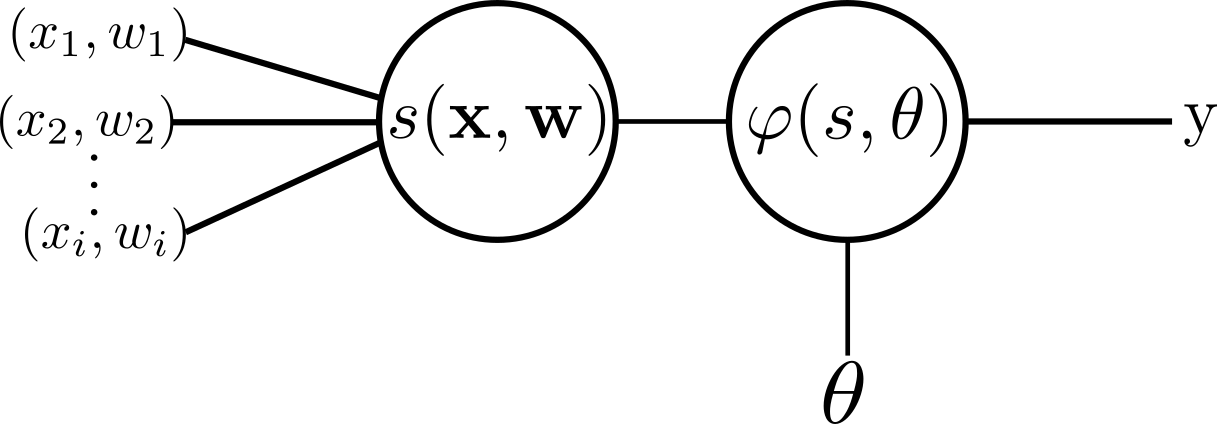
\includegraphics[width=0.6\textwidth]{images/PittsMcCulloch.png}
    \caption{Model neuronu Pittsa-McCullocha}
    \label{fig:pitts}
\end{figure}

\section{Przykład dwóch rysunków obok siebie}

\begin{figure}[htbp]
    \centering
    \begin{minipage}{0.48\textwidth}
        \centering
        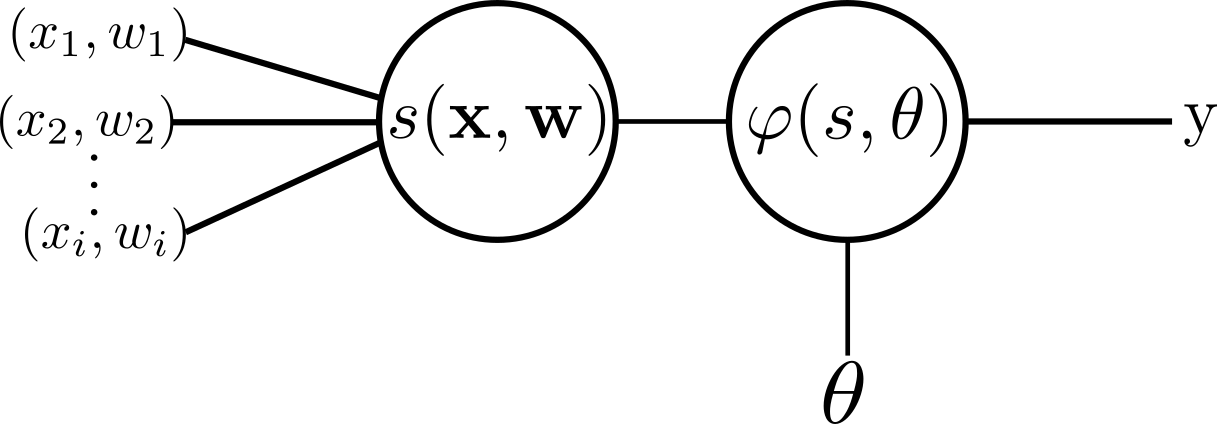
\includegraphics[width=\textwidth]{images/PittsMcCulloch.png}
        \caption{Model neuronu -- wariant A}
        \label{fig:pitts_a}
    \end{minipage}
    \hfill
    \begin{minipage}{0.48\textwidth}
        \centering
        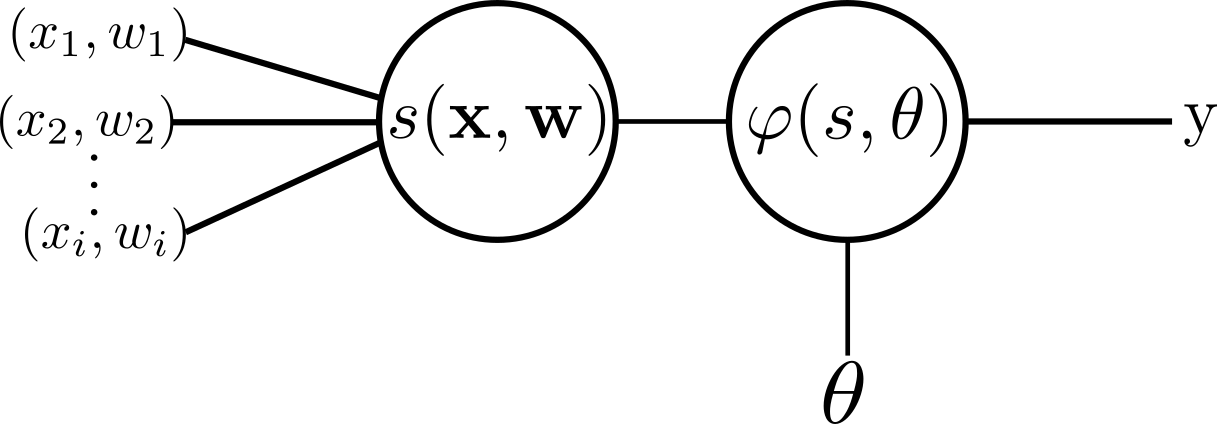
\includegraphics[width=\textwidth]{images/PittsMcCulloch.png}
        \caption{Model neuronu -- wariant B}
        \label{fig:pitts_b}
    \end{minipage}
\end{figure}

\section{Przykład tabeli}

\begin{table}[htbp]
    \centering
    \caption{Porównanie wybranych parametrów}
    % warto użyć https://www.tablesgenerator.com
    \label{tab:parametry}
    \begin{tabular}{|l|c|c|}
        \hline
        \textbf{Parametr} & \textbf{Wartość A} & \textbf{Wartość B} \\
        \hline
        Dokładność        & 0.95               & 0.89               \\
        Precyzja          & 0.93               & 0.87               \\
        Czułość           & 0.91               & 0.85               \\
        F1-score          & 0.92               & 0.86               \\
        \hline
    \end{tabular}
\end{table}

\section{Przykład listingu -- Python}

\begin{lstlisting}[language=Python, caption={Hello World w Pythonie}, label={lst:python}]
print("Hello, World!")
\end{lstlisting}

\section{Przykład listingu -- C}

\begin{lstlisting}[language=C, caption={Hello World w C}, label={lst:c}]
#include <stdio.h>

int main(void) {
    printf("Hello, World!\n");
    return 0;
}
\end{lstlisting}

\section{Przykładowe równania}
Przykładowe równanie przedstawiono na \eqref{eq:Intro:DeltaRule},
\begin{equation} \label{eq:Intro:DeltaRule}
    \Delta \vec{w_j} = \eta \epsilon_j f'(s_j) \vec{x_j} = \eta (t_j - y_j) f'(\vec{w_{j-1}}^T \vec{x_j}) \vec{x_j}
\end{equation}
podczas gdy zbiór równań przedstawiono na \eqref{eq:Intro:GiniEntropy}
\begin{equation} \label{eq:Intro:GiniEntropy}
    \begin{split}
        H &= - \sum_i p_i log(p_i) \\
        G &= 1 - \sum_i p_i^2.
    \end{split}
\end{equation}


%%%%%%%%%%%%%%%%%%%%%%%%%%%%%%%%%%%%%%%%
\chapter{Wyniki} \label{ch:wyniki}
Lorem ipsum dolor sit amet, consectetur adipiscing elit, sed do eiusmod tempor incididunt ut labore et dolore magna aliqua. Odio pellentesque diam volutpat commodo sed. Proin fermentum leo vel orci porta non pulvinar neque laoreet. Diam volutpat commodo sed egestas egestas fringilla. Elit at imperdiet dui accumsan sit amet nulla. Vel pretium lectus quam id leo in vitae. Faucibus vitae aliquet nec ullamcorper sit amet risus. Leo vel fringilla est ullamcorper eget nulla facilisi etiam dignissim. Quis risus sed vulputate odio ut enim blandit volutpat. Tempor commodo ullamcorper a lacus vestibulum. Tincidunt augue interdum velit euismod. Ullamcorper dignissim cras tincidunt lobortis feugiat. A condimentum vitae sapien pellentesque habitant morbi tristique senectus. Volutpat ac tincidunt vitae semper quis lectus nulla at. Tortor aliquam nulla facilisi cras fermentum odio eu feugiat. Leo integer malesuada nunc vel risus. Turpis in eu mi bibendum neque egestas congue quisque. Mattis rhoncus urna neque viverra justo nec ultrices dui. Lorem sed risus ultricies tristique nulla. Vitae tortor condimentum lacinia quis vel eros.

%%%%%%%%%%%%%%%%%%%%%%%%%%%%%%%%%%%%%%%%
\chapter{Podsumowanie} \label{ch:podsumowanie}
Lorem ipsum dolor sit amet, consectetur adipiscing elit, sed do eiusmod tempor incididunt ut labore et dolore magna aliqua. Odio pellentesque diam volutpat commodo sed. Proin fermentum leo vel orci porta non pulvinar neque laoreet. Diam volutpat commodo sed egestas egestas fringilla. Elit at imperdiet dui accumsan sit amet nulla. Vel pretium lectus quam id leo in vitae. Faucibus vitae aliquet nec ullamcorper sit amet risus. Leo vel fringilla est ullamcorper eget nulla facilisi etiam dignissim. Quis risus sed vulputate odio ut enim blandit volutpat. Tempor commodo ullamcorper a lacus vestibulum. Tincidunt augue interdum velit euismod. Ullamcorper dignissim cras tincidunt lobortis feugiat. A condimentum vitae sapien pellentesque habitant morbi tristique senectus. Volutpat ac tincidunt vitae semper quis lectus nulla at. Tortor aliquam nulla facilisi cras fermentum odio eu feugiat. Leo integer malesuada nunc vel risus. Turpis in eu mi bibendum neque egestas congue quisque. Mattis rhoncus urna neque viverra justo nec ultrices dui. Lorem sed risus ultricies tristique nulla. Vitae tortor condimentum lacinia quis vel eros.

%%%%%%%%%%%%%%%%%%%%%%%%%%%%%%%%%%%%%%%%
 % opcjonalne
\symbolslist{
    $a$ -- (mała litera kursywą)  skalar

    $\bm{a}$ -- (mała pogrubiona litera) wektor,

    $\bm{A}$ -- (wielka pogrubiona litera) macierz

    $\bm{A_i}$ -- $i$-ty wiersz macierzy - wektor

    $a_i$ -- $i$-ty element wektora - skalar

    $\mathbb{B}$ -- zbiór liczb binarnych $\{0, 1\}$

    $\pm \mathbb{B}$ -- zbiór liczb bipolarnych $\{-1, 1\}$
}
 % opcjonalne
\abbreviationslist{
    PŁ -- Politechnika Łódzka
    
    AI -- sztuczna inteligencja
}
 % opcjonalne
\definitionslist{
    Sepulka –- l.mn. sepulki, odgrywający doniosłą rolę element cywilizacji Ardrytów (ob.) z planety Enteropii (ob.). Ob. sepulkaria.

    Sepulkaria –- l.poj. sepulkarium, obiekty służące do sepulenia (ob.).

    Sepulenie –- czynność Ardrytów (ob.) z planety Enteropii (ob.). Ob. sepulki. Źródło: Stanisław Lem, Dzienniki gwiazdowe – Podróż czternasta.
    % https://pl.wikipedia.org/wiki/Sepulka
}

 % opcjonalne
\addattachment{Przykładowy załącznik LaTeX}{Lorem ipsum dolor sit amet, consectetur adipiscing elit, sed do eiusmod tempor incididunt ut labore et dolore magna aliqua. Odio pellentesque diam volutpat commodo sed. Proin fermentum leo vel orci porta non pulvinar neque laoreet. Diam volutpat commodo sed egestas egestas fringilla. Elit at imperdiet dui accumsan sit amet nulla. Vel pretium lectus quam id leo in vitae. Faucibus vitae aliquet nec ullamcorper sit amet risus. Leo vel fringilla est ullamcorper eget nulla facilisi etiam dignissim. Quis risus sed vulputate odio ut enim blandit volutpat. Tempor commodo ullamcorper a lacus vestibulum. Tincidunt augue interdum velit euismod. Ullamcorper dignissim cras tincidunt lobortis feugiat. A condimentum vitae sapien pellentesque habitant morbi tristique senectus. Volutpat ac tincidunt vitae semper quis lectus nulla at. Tortor aliquam nulla facilisi cras fermentum odio eu feugiat. Leo integer malesuada nunc vel risus. Turpis in eu mi bibendum neque egestas congue quisque. Mattis rhoncus urna neque viverra justo nec ultrices dui. Lorem sed risus ultricies tristique nulla. Vitae tortor condimentum lacinia quis vel eros.

Lorem ipsum dolor sit amet, consectetur adipiscing elit, sed do eiusmod tempor incididunt ut labore et dolore magna aliqua. Odio pellentesque diam volutpat commodo sed. Proin fermentum leo vel orci porta non pulvinar neque laoreet. Diam volutpat commodo sed egestas egestas fringilla. Elit at imperdiet dui accumsan sit amet nulla. Vel pretium lectus quam id leo in vitae. Faucibus vitae aliquet nec ullamcorper sit amet risus. Leo vel fringilla est ullamcorper eget nulla facilisi etiam dignissim. Quis risus sed vulputate odio ut enim blandit volutpat. Tempor commodo ullamcorper a lacus vestibulum. Tincidunt augue interdum velit euismod. Ullamcorper dignissim cras tincidunt lobortis feugiat. A condimentum vitae sapien pellentesque habitant morbi tristique senectus. Volutpat ac tincidunt vitae semper quis lectus nulla at. Tortor aliquam nulla facilisi cras fermentum odio eu feugiat. Leo integer malesuada nunc vel risus. Turpis in eu mi bibendum neque egestas congue quisque. Mattis rhoncus urna neque viverra justo nec ultrices dui. Lorem sed risus ultricies tristique nulla. Vitae tortor condimentum lacinia quis vel eros.

Lorem ipsum dolor sit amet, consectetur adipiscing elit, sed do eiusmod tempor incididunt ut labore et dolore magna aliqua. Odio pellentesque diam volutpat commodo sed. Proin fermentum leo vel orci porta non pulvinar neque laoreet. Diam volutpat commodo sed egestas egestas fringilla. Elit at imperdiet dui accumsan sit amet nulla. Vel pretium lectus quam id leo in vitae. Faucibus vitae aliquet nec ullamcorper sit amet risus. Leo vel fringilla est ullamcorper eget nulla facilisi etiam dignissim. Quis risus sed vulputate odio ut enim blandit volutpat. Tempor commodo ullamcorper a lacus vestibulum. Tincidunt augue interdum velit euismod. Ullamcorper dignissim cras tincidunt lobortis feugiat. A condimentum vitae sapien pellentesque habitant morbi tristique senectus. Volutpat ac tincidunt vitae semper quis lectus nulla at. Tortor aliquam nulla facilisi cras fermentum odio eu feugiat. Leo integer malesuada nunc vel risus. Turpis in eu mi bibendum neque egestas congue quisque. Mattis rhoncus urna neque viverra justo nec ultrices dui. Lorem sed risus ultricies tristique nulla. Vitae tortor condimentum lacinia quis vel eros.

Lorem ipsum dolor sit amet, consectetur adipiscing elit, sed do eiusmod tempor incididunt ut labore et dolore magna aliqua. Odio pellentesque diam volutpat commodo sed. Proin fermentum leo vel orci porta non pulvinar neque laoreet. Diam volutpat commodo sed egestas egestas fringilla. Elit at imperdiet dui accumsan sit amet nulla. Vel pretium lectus quam id leo in vitae. Faucibus vitae aliquet nec ullamcorper sit amet risus. Leo vel fringilla est ullamcorper eget nulla facilisi etiam dignissim. Quis risus sed vulputate odio ut enim blandit volutpat. Tempor commodo ullamcorper a lacus vestibulum. Tincidunt augue interdum velit euismod. Ullamcorper dignissim cras tincidunt lobortis feugiat. A condimentum vitae sapien pellentesque habitant morbi tristique senectus. Volutpat ac tincidunt vitae semper quis lectus nulla at. Tortor aliquam nulla facilisi cras fermentum odio eu feugiat. Leo integer malesuada nunc vel risus. Turpis in eu mi bibendum neque egestas congue quisque. Mattis rhoncus urna neque viverra justo nec ultrices dui. Lorem sed risus ultricies tristique nulla. Vitae tortor condimentum lacinia quis vel eros.}

\addpdfattachment{Przykładowy załącznik pdf - wymogi edycyjne}{attachments/WymogiEdycyjne.pdf}

\end{document}